
% ======================================================================
% starting package maintenance...
% installation directory: "C:\Users\Bernardo Goncalves\AppData\Local\Programs\MiKTeX"
% package repository: https://mirror.kku.ac.th/CTAN/systems/win32/miktex/tm/packages/
% package repository digest: bc26c9dcac319ee10e5af84d3734de2b
% going to download 69253 bytes
% going to install 43 file(s) (1 package(s))
% downloading https://mirror.kku.ac.th/CTAN/systems/win32/miktex/tm/packages/latexindent.tar.lzma...
% 0.07 MB, 0.24 Mbit/s
% extracting files from latexindent.tar.lzma...
% ======================================================================
\documentclass[11pt]{article}
% Language setting
% Replace `english' with e.g. `spanish' to change the document language
\usepackage[english]{babel}
% Set page size and margins
% Replace `letterpaper' with `a4paper' for UK/EU standard size
\usepackage[a4paper,top=2cm,bottom=2cm,left=3cm,right=3cm,marginparwidth=1.75cm]{geometry}
% Useful packages
\usepackage{amsmath}
\usepackage{graphicx}
\usepackage{subcaption}
\usepackage{booktabs}
\usepackage{multirow}
\usepackage{array}
\usepackage[nottoc]{tocbibind}
\usepackage[backend=bibtex,style=ieee]{biblatex}
\addbibresource{adrenal.bib}
\usepackage[colorlinks=true, allcolors=blue]{hyperref}

\title{A Review of Adrenal Lesions Diagnosis with Machine Learning}
\author{Bernardo Gonçalves}
\providecommand{\keywords}[1]{  \small  \textbf{\textit{Keywords---}} #1}




\begin{document}
\maketitle

\begin{abstract}

    Adrenal glands play a vital role in maintaining homeostasis under chronic
    stressors. They are susceptible to a range of malignant and benign lesions,
    including adrenal adenomas, which are the most common lesions. The
    diagnosis of these lesions is made via conventional imaging techniques, such
    as magnetic resonance imaging and computed tomography, is complex and
    depends heavily on the radiologist's knowledge and experience. Misdiagnosis due to the
    presence of pseudo lesions, imaging features overlap, or incorrect technique
    selection can lead to unnecessary costs and examinations, as most adrenal
    lesions do not require treatment. Machine learning methods have been
    proposed to improve adrenal lesion diagnosis.
    In this paper, we analyse all
    studies from 2017 until September 2022 that aim to diagnose or differentiate
    adrenal lesions using MRI or CT scans and machine learning methods. 
    The studies that were not written in
    English, that were state-of-the-art reviews, that did not report which
    machine learning model was used, or that did not have the full text
    available were excluded from our analysis. For the sake of clarity, we
    divided our analysis into three categories accordingly to the goal of the
    studies: differentiation between adrenal adenomas and other lesions,
    differentiation between benign and malignant lesions, and studies that did
    not fit in any of the other groups. Despite the promising results that were
    reported, our analysis highlights the lack of deep learning studies,
    prospective studies, multicenter validations, and comparisons between the
    performance of the machine learning model and the radiologist's performance.
    Therefore, this paper serves as a comprehensive review of the current
    state-of-the-art in ML-based adrenal lesion diagnosis, while also
    identifying important research gaps that require further investigation.

\end{abstract}

\keywords{Adrenal, Lesions, Machine Learning, Diagnosis, MRI, CT, Detection}

\section{Introduction}

The adrenal glands, or suprarenal glands, are a component of the
Hypothalamic-Pituitary-Adrenal (HPA) axis, which is responsible to maintain
homeostasis in the presence of chronic stressors, activating a complex range of
responses from the endocrine, nervous and immune systems, generally known as the
stress response \cite{open}.

The adrenal glands can be affected by a wide variety of benign and malignant
lesions. Approximately 9\% of the global population is estimated to have adrenal
lesions, which are mostly detected incidentally during abdominal imaging
\cite{Dhamija2015}. Adrenal adenomas represent 50 to 80\% of all adrenal lesions
\cite{Bracci2022}. 
Adenomas are often non-functional and remain asymptomatic, being discovered incidentally
\cite{Platzek2019}. Adrenocortical carcinomas, despite being the most common
primary adrenal lesion, are very rare, representing only 0.7–2.0 cases per million
habitants per year \cite{Bracci2022}. 
Also, the adrenals are a frequent location of metastases \cite{Platzek2019},
approximately 25\% of patients with cancer have adrenal metastases on autopsy
\cite{Bracci2022}.

In general, non-functional lesions do not require any treatment, therefore it is
crucial to differentiate between adenomas (typical non-functional lesions) and
non-adenomas \cite{Platzek2019}, to avoid unnecessary treatment.
Commonly, adrenal adenomas have less than 1 cm in
diameter and they can be lipid-rich or lipid-poor \cite{Panda2015}.
About 70-80 \% of the adenomas are lipid-rich in contrast with the malignant
lesions \cite{Platzek2019}. This results in a 20-30 \% overlap between adenomas
and malignant lesions in terms of intracytoplasmic lipid content
\cite{Israel2004}.

% Adrenal Imaging - medical diagnosis of adrenal lesions

Structural medical imaging techniques are decisive in detecting and
characterising adrenal lesions and complementary to functional imaging and
endocrine evaluation in the assessment of functional lesions. Imaging techniques
can also rule out invasive interventions. The most used imaging techniques to
evaluate the adrenal glands are Computed Tomography (CT) and Magnetic Resonance
Imaging (MRI) \cite{Panda2015}.

Figure \ref{fig:adrenal_glands_normal} shows the V- (left) and Y-shaped (right)
normal glands. Figure \ref{fig:adrenal_ct} is an axial contrast-enhanced CT
image in the arterial phase where both glands are enhanced due to the high
retroperitoneal fat content. Figure \ref{fig:adrenal_mri} is a coronal MR
Chemical Shift Image (CSI) out-of-phase showing normal adrenal glands as well.

\begin{figure}
    \centering
    \begin{subfigure}[b]{0.45\textwidth}
        \centering
        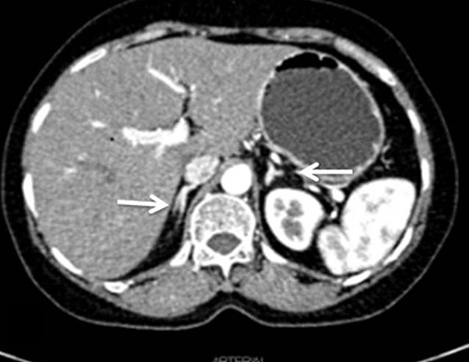
\includegraphics[width=\textwidth]{figures/CT_adrenal_enhanced.png}
        \caption{Adrenal glands in a contrast-enhanced CT axial slice in the arterial phase. Due to the high level of retroperitoneal fat, both glands are enhanced in this image slice. Reprinted from \cite{Panda2015}.}
        \label{fig:adrenal_ct}
    \end{subfigure}
    \hfill
    \begin{subfigure}[b]{0.45\textwidth}
        \centering
        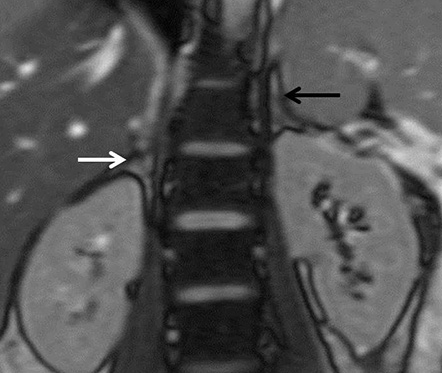
\includegraphics[width=\textwidth]{figures/MRI_adrenal.png}
        \caption{Adrenal glands in an MR CSI coronal slice. Both glands have an intermediate signal intensity. Reprinted from \cite{Panda2015}. }
        \label{fig:adrenal_mri}
    \end{subfigure}
    \caption{Normal adrenal glands in CT and MR slices. The arrows indicate the localization of the glands.}
    \label{fig:adrenal_glands_normal}
\end{figure}

The differential diagnosis between adenomas and non-adenomas is
of extreme importance. This diagnosis can be hindered by the existence of
lipid-poor adenomas that are more difficult to diagnose. Lipid-rich adenomas can
be easily identified using unenhanced CT (less than 10 HU) \cite{Panda2015} or CSI
\cite{Platzek2019}. However, unenhanced CT is not indicated to detect lipid-poor
adenomas \cite{Israel2004}. In these cases, CSI presents itself as a better
solution because of its improved sensitivity to low levels of lipid content and
therefore it can detect 62-67\% of the adenomas uncharacterized by unenhanced CT
\cite{Israel2004}.

CSI is a fat-suppression technique that originates two sets of images: in-phase
(IP) and out-of-phase (OP) images. In OP images the signal is the difference
between the signals of water and fat molecules. In IP images the signal of both
water and fat is added. Thus, there is a significant suppression of the signal
from IP to OP images in lipid-rich lesions \cite{Jahanvi2021}. OP images are
characterised by the so-called India ink artefact, which is a signal void in the
margins of fatty and normal tissues \cite{Jahanvi2021}, creating a darker
boundary in lipid-rich lesions such as most adenomas. Figure \ref{fig:adenomas}
shows two adenomas, one lipid-rich (up) and the other lipid-poor (down) using
CSI. The red boxes surround the adenomas. The
signal difference in the region of the lesion between IP and OP images is much greater in lipid-rich
adenomas than in lipid-poor adenomas, facilitating the diagnostic process of
lipid-rich adenomas. Given these images, the diagnosis of
adenoma can be made by visual evaluation or by quantitative indices such as the
adrenal Signal Intensity Index (SII), Adrenal-to-Spleen Ratio (ASR),
Adrenal-to-Liver Ratio (ALR) or the Adrenal-to-Muscle Ratio (AMR)
\cite{Fujiyoshi2003}. A metanalysis with 1280
lesions (859 adenomas, 421 non-adenomas) documented a sensitivity of 94\% and
a specificity of 95\% in detecting adrenal adenomas with the CSI technique using
visual evaluation and/or quantitative methods \cite{Platzek2019}. Despite the
elevated values, the authors assert that lipid-poor adenomas continue to present
challenges, even when employing CSI. 

\begin{figure}
    \centering
    \begin{subfigure}[b]{0.45\textwidth}
        \centering
        \includegraphics[width=\textwidth]{figures/S016_I027_93033860_Axial_GR-['SS','SP','SK']-UNKNOWN_no_60_70.png}
        \caption{T1-weighted out-of-phase axial slice with a lipid-rich adenoma.}
        \label{fig:adenoma_lr_OP}
    \end{subfigure}
    \hfill
    \begin{subfigure}[b]{0.45\textwidth}
        \centering
        \includegraphics[width=\textwidth]{figures/S016_I028_93033860_Axial_GR-['SS','SP','SK']-UNKNOWN_no_60_70.png}
        \caption{T1-weighted in-phase axial slice with a lipid-rich adenoma.}
        \label{fig:adenoma_lr_IP}
    \end{subfigure}
    \vfill
    \begin{subfigure}[b]{0.45\textwidth}
        \centering
        \includegraphics[width=\textwidth]{figures/S003_I023_93036417_Axial_GR-['SS','SP','SK']-UNKNOWN_no_70_80.png}
        \caption{T1-weighted out-of-phase axial slice with a lipid-poor adenoma.}
        \label{fig:adenoma_lp_OP}
    \end{subfigure}
    \hfill
    \begin{subfigure}[b]{0.45\textwidth}
        \centering
        \includegraphics[width=\textwidth]{figures/S003_I024_93036417_Axial_GR-['SS','SP','SK']-UNKNOWN_no_70_80.png}
        \caption{T1-weighted in-phase axial slice with a lipid-poor adenoma.}
        \label{fig:adenoma_lp_IP}
    \end{subfigure}
    \caption{Adrenal adenomas in axial MR CSI. The red rectangles surround the adenomas. Lipid-rich adenomas have a much greater intensity difference between in-phase and out-of-phase images.   }
    \label{fig:adenomas}
\end{figure}

When analysing lipid-poor adenomas, the addition of Dynamic Contrast-Enhanced (DCE) sequences is
favourable, increasing the diagnostic performance \cite{Barat2022}. In
\cite{Chung2001} 35 adrenal adenomas were analysed and it was concluded that the
enhancement pattern of the adenomas is different from the one presented by
malignant lesions. Adenomas present a homogeneous capillary blush in 18 seconds
post-gadolinium images and a rapid washout in 45 seconds post-gadolinium images.
In \cite{Platzek2019} it was concluded that the
quantitative methods do not present a significant advantage to the visual
diagnosis. In addition, the authors do not recommend any additional imaging if
the adenoma diagnosis is confirmed based on CSI. However, if the adenoma is not
confirmed, DCE sequences would help distinguish between adenomas and
malignant lesions \cite{Platzek2019}.

% Machine learning - for adrenal lesion

The growing number of abdominal imaging studies has led to the increasing
frequency of adrenal incidentalomas, which are usually benign, non-functional
adenomas. Nevertheless, it is important to evaluate their functional status and
malignancy, as soon as possible. The diagnosis of adrenal
lesions is a complex process that involves both biochemical and radiological
evaluation \cite{Anagnostis2009}. Adrenal radiologic evaluation via conventional
imaging is a challenging process that depends largely on the experience and
knowledge of the radiologist \cite{Zhang2022}. Several pitfalls can result in the
misdiagnosis of adrenal lesions, such as the presence of pseudo lesions, overlap
of imaging features of different lesions, or incorrect choice of the imaging
technique \cite{Elsayes2020}. New approaches to the diagnosis of adrenal lesions
are crucial to avoid misdiagnosis, which can lead to increased treatment costs
or unnecessary examination \cite{Zhang2022}. Additionally, it would be important
to decrease the number of imaging exams that are necessary to complete the
diagnosis. Machine learning methods have been proposed as a potential solution
not only to improve the diagnostic accuracy and efficiency of adrenal lesions. Most of these machine learning methods analyse medical
imaging features extracted using radiomic methods that will be briefly explored
in \ref{subsec:radiomic}.

% Radiomics

Radiomics is the extraction of quantitative features from medical images, such
as Positron Emission Tomography (PET), MRI, or CT. Before the feature extraction
is necessary to limit the amount of data that needs to be processed in order to
extract features - ROI (region of interest) segmentation. This process can be manual, which is the gold
standard, where a specialist selects the ROI. Manual segmentation is a
time-consuming task that significantly depends on the skill of the operator.
There are fully automatic methods for ROI segmentation however, they can fail in
difficult cases, such as lesions with indistinct borders and are highly
dependent on the quality of the image. For that reason, the usage of
semi-automatic methods is preferable. These methods have minimal user
interaction (seed identification or manual correction). The extracted
quantitative features aim to describe the complexity of the individual region of
interest. Ordinarily, these features are divided into 4 categories:

\begin{enumerate}
    \item Shape-Based Features: numeric information respecting geometrics characteristics, like shape and size.
    \item First-Order Statistics: distribution of voxel values without spatial information, generally histogram-based.
    \item Second-Order Statistics: “texture” features, focus on the spatial relationships between voxels with similar grey levels.
    \item High-Order Statistics: usage of filters to extract patterns from the images. From the resultant images, first and second-order features are extracted.
\end{enumerate}

The most relevant radiomic features to the task in hand are selected using
statistical approaches or machine learning \cite{Zhang2022}. Then, these
features are used as the input of ML models to classify the region of interest.
This type of workflow is widespread, appearing in 87\% (20/23) of the analysed
studies. Traditional machine learning models like K-means, Support Vector
Machine (SVM), Logistic Regression (LogReg), or Random Forest (RanFor), are
frequently used to classify radiomic features of regions of interest and have
achieved high performance in different anatomical regions \cite{Zhang2022,
    Wagner2021}. Deep Learning models, such as Convolutional Neural Networks
(CNNs), have been often applied to medical images from several anatomical
regions with promising results \cite{Anaya-Isaza2021}. Despite that, only 13\%
of the presented studies report the application of DL models to
adrenal images. DL models are different from ML models mostly because they
demand bigger annotated data sets and they do not rely on the feature extraction
step (all features are automatically extracted and classified by the model).

\section{Methods}

The studies analysed in this section were selected according to the following PICO criteria:

\begin{enumerate}
    \item[] \textbf{P (patients) }– patients with adrenal lesions.
    \item[] \textbf{I (interventions) }– machine learning (including deep learning) modelling.
    \item[] \textbf{C (comparison) }– standard of care imaging including Computed Tomography (CT) and Magnetic Imaging Resonance (MRI).
    \item[] \textbf{O (outcome) }– lesion differentiation (benign/malign and subtyping) and lesions detection.
\end{enumerate}

The studies were obtained by searching PubMed and Web of Science databases in
June 2023. The following research string was used: (adrenal
or suprarenal) AND (CT OR "computed tomography" OR MRI OR "magnetic resonance
imaging" OR "MRI scan" OR "nuclear magnetic resonance" OR "magnetic resonance"
OR NMR) AND ("deep learning" OR "convolutional networks" OR CNN OR "neural
networks" OR convolutional OR DNN OR SVM OR "Support vector machine" OR
"decision tree" OR "machine learning"). Studies that were: (a) reviews, (b) not
written in English, (c) did not report a modelling method, (d) did not have the
full text available were excluded from this research. The publication dates of
the studies range from 2017 until June 2023.

The research resulted in 23 studies that were divided into 3 groups according with
their object of study:
\begin{enumerate}
    \item[] \textbf{Group A}: contains all the studies that focus on the
        differentiation between adrenal adenomas and other adrenal lesions.
    \item[] \textbf{Group B}: contains all the studies that target the
        differentiation between benign and malignant adrenal lesions.
    \item[] \textbf{Group C}: contains the remaining studies that did not fit
        any of the above categories.
\end{enumerate}
Table \ref{tab:sota_sum} shows the distribution of the selected studies in terms
of their group, image modality and model type. Overall, most of the studies
adopt traditional machine learning models to classify imaging features
(radiomics) from CT images to distinguish adenomas from other types of adrenal
lesions, eg. Metastases, pheochromocytomas.

\begin{table}[h]
    \centering
    \begin{tabular}{cccccccc}\toprule
        \multirow{2}{*}{\textbf{Group}} & \multicolumn{3}{c}{\textbf{Image Modality}} & \multicolumn{3}{c}{\textbf{Model Type}} & \multirow{2}{*}{\textbf{Total}}
        \\\cmidrule(lr){2-4} \cmidrule(lr){5-7}
                                        & \textbf{MRI}                                & \textbf{CT}                             & \textbf{MRI+CT}                 & \textbf{ML} & \textbf{DL} & \textbf{ML+DL}      \\\midrule
        A - Adenomas vs other lesions   & 4                                           & 7                                       & 1                               & 11          & 1           & 0              & 12 \\
        B - Benign vs Malign            & 2                                           & 5                                       & 0                               & 7           & 0           & 0              & 7  \\
        C - Other                       & 1                                           & 3                                       & 0                               & 2           & 1           & 1              & 4  \\
        Sum                             & 7                                           & 15                                      & 1                               & 20          & 2           & 1              & 23 \\
        \bottomrule
    \end{tabular}
    \caption{Studies distribution per group. CT: Computed Tomography; MRI: Magnetic Resonance Imaging; ML: Traditional Machine Learning; DL: Deep Learning.}
    \label{tab:sota_sum}
\end{table}

In the next 3 sections, each group of papers will be analysed in detail,
exploring their common and contrasting aspects. For each group, the analysis
will be focused on the utilized data sets, models, and the obtained results.

\section{Results}

\subsection{Group A - Adenomas vs other lesions}

Group A comprises all studies that focus on the differentiation between adenomas
and other lesions. This group corresponds to 52\% of all analysed studies.
Tables \ref{tab:data_A}, \ref{tab:model_A} and \ref{tab:res_A} present an
overview of the data sets, models, and results, respectively, for each study
within group A.

Adenomas are the common lesion in all of these studies and they are compared
with three different lesions: metastases \cite{Schieda2017,Tu2018,Tu2020};
pheochromocytomas \cite{Yi20181,Yi2018, Liu2022,Liu2021}, and carcinomas
\cite{Elmohr2019, Torresan2021, Ho2019}. In \cite{Tu2020, Yi2018, Yi20181,
    Liu2022} the data sets of adenomas consisted only in lipid-poor adenomas. Only
one study had a non-binary data set with 3 classes: \cite{Romeo2018} data set
has 3 classes: lipid-poor adenomas, lipid-rich adenomas and non-adenomas. The
author of \cite{Kusunoki2022} do not specify another lesion type, performing
differentiation between adenomas and non-adenomas. Most of the data sets (8 of
12 studies) contain CT images. From those, 6 use both images with and without
contrast. The remaining have MRI datasets, all with CSI and T2W images. The
sample size of the studies ranges from dozens to hundreds of lesions, which is
closely related to the applied inclusion criteria and the initial sample size.
For example, one study had a database of 336 patients however only 19 met the
inclusion criteria, each with one lesion \cite{Torresan2021}. Most of the
presented data sets are unbalanced with a much higher number of adenomas.

All studies, except one, performed lesion classification
with ML models using radiomic features. The most frequent model is logistic
regression (LogReg), followed by the support vector machine (SVM) and decision
tree-based models. In every study, the region of interest (ROI) was manually
selected by experts. The extraction of first and second-order statistics is a
widespread practice, but only 3 studies extracted shape-based features, and none
extracted higher-order statistics. The only study that has implemented a DL
model has performed ROI (selected, cropped and labelled by experts)
classification with a deep convolution neural network \cite{Kusunoki2022}. They
reported the usage of augmentation techniques such as rotations and horizontal
flips. There is only one study that implemented an unsupervised model (K-means) \cite{Torresan2021}.

In \cite{Ho2019} the data set consists of lipid-poor adenomas and
carcinomas in both MRI and CT images. The objective of this work was to compare
the different image modalities using the same machine learning approach. The
authors have reported only the Area Under the Receiving Operating Characteristic
Curve (AUC). The value presented in Table \ref{tab:res_A} refers to the best result,
using CE-CT images and with MRI images the value decreases to 58 \%.

Both works by Yi et al \cite{Yi2018, Yi20181} implemented a logistic regression
model with the same radiomic features but using different CT images and achieved
impressive results. However, \cite{Yi2018} adds clinical features such as
necrosis or calcification and lesion dimensions, to the radiomic features. Also,
to improve feature selection the authors used the Least Absolute Shrinkage and
Selection Operator (LASSO). These studies achieved the best results for this
group. However, in terms of sensitivity, a higher
value was obtained by \cite{Yi2018}. Overall, there are 4 studies in which their metrics average more than
90\%: \cite{Yi2018, Yi20181, Kusunoki2022, Schieda2017}. Three of them use CT
images. \cite{Schieda2017} had a very small unbalanced dataset and used CSI
images to differentiate renal cell carcinomas from adenomas.


\begin{table}[]
    \centering
    \begin{tabular}{ccccc}\toprule
        \multirow{2}{*}{\textbf{Reference}} & \multirow{2}{*}{\textbf{Image Modality}} & \multicolumn{3}{c}{\textbf{Sample Size (lesions)}}
        \\\cmidrule(lr){3-5}
                                            &                                          & \textbf{Total}                                     & \textbf{Adenomas} & \textbf{Other} \\\midrule
        \cite{Tu2018}                       & U-CT                                     & 76                                                 & 36                & 40             \\
        \cite{Yi20181}                      & U/CE-CT                                  & 110                                                & 80                & 30             \\
        \cite{Yi2018}                       & U-CT                                     & 265                                                & 181               & 84             \\
        \cite{Elmohr2019}                   & CE-CT                                    & 54                                                 & 25                & 29             \\
        \cite{Torresan2021}                 & U/CE-CT                                  & 19                                                 & 9                 & 10             \\
        \cite{Kusunoki2022}                 & U/CE-CT                                  & 115                                                & 83                & 32             \\
        \cite{Liu2022}                      & U/CE-CT                                  & 280                                                & 188               & 92             \\
        \cite{Ho2019}                       & U/CE-CT; T1W-OP/IP MRI                   & 23                                                 & 15                & 8              \\
        \cite{Liu2021}                      & T1W-OP/IP; T2W MRI                       & 60                                                 & 40                & 20             \\
        \cite{Schieda2017}                  & T1W-OP/IP; T2W MRI                       & 44                                                 & 29                & 15             \\
        \cite{Tu2020}                       & T1W-OP/IP; T2W MRI                       & 63                                                 & 23                & 40             \\
        \cite{Romeo2018}                    & T1W-OP/IP; T2W MRI                       & 60                                                 & 40                & 20
        \\\bottomrule
    \end{tabular}
    \caption{Dataset Details for each article in Group A. CT: Computed Tomography; U: Unenhanced; CE: Contrast Enhanced; MRI: Magnetic Resonance Imaging; OP: Out-of-phase; IP: In-phase; T1W: T1-weighted; T2W: T2-weighted.}
    \label{tab:data_A}
\end{table}

\begin{table}[]
    \centering
    \begin{tabular}{cccccc}\toprule
        \multirow{2}{*}{\textbf{Reference}} & \multirow{2}{*}{\textbf{Type}} & \multirow{2}{*}{\textbf{Classification Model}} & \multirow{2}{*}{\textbf{ROI}} & \multirow{2}{*}{\textbf{Features}} \\
        \\\midrule
        \cite{Tu2018}                       & ML                             & LogReg                                         & Manual                        & $1^{st}$                           \\
        \cite{Yi20181}                      & ML                             &
        LogReg                              & Manual                         & $1^{st}$, $2^{nd}$, higher                                                                                          \\
        \cite{Yi2018}                       & ML                             &
        LogReg                              & Manual
                                            & $1^{st}$, $2^{nd}$, higher                                                                                                                           \\
        \cite{Elmohr2019}                   & ML                             & RanFor; LogReg                                 & Manual                        & $1^{st}$, $2^{nd}$, shape          \\
        \cite{Torresan2021}                 & ML                             & K-Means                                        & Manual                        & $1^{st}$, $2^{nd}$                 \\
        \cite{Kusunoki2022}                 & DL                             & DCNN                                           & Manual                        & -                                  \\
        \cite{Liu2022}                      & ML                             & LinReg; SVM; RanFor                            & Manual                        & $1^{st}$; clinical                 \\
        \cite{Ho2019}                       & ML                             & LogReg                                         & Manual                        & $1^{st}$, $2^{nd}$, shape          \\
        \cite{Liu2021}                      & ML                             & SVM                                            & Manual                        & $1^{st}$                           \\
        \cite{Schieda2017}                  & ML                             & LogReg                                         & Manual                        & $1^{st}$                           \\
        \cite{Tu2020}                       & ML                             & LogReg                                         & Manual                        & $1^{st}$, shape                    \\
        \cite{Romeo2018}                    & ML                             & DecTre                                         & Manual                        & $1^{st}$, $2^{nd}$                 \\
        \bottomrule
    \end{tabular}
    \caption{Modelling Details for each article in the Group A. ML: Traditional Machine Learning models; DL: Deep Learning models; LogReg: Logistic Regression; LASSO: Least Absolute Shrinkage and Selection Operator; DecTre: Decision Tree; RanFor: Random Forest; PCA: Principal Components Analysis; SVM: Support Vector Machine; $1^{st}$, $2^{nd}$, higher: first, second, higher order statistics, respectively; shape: shape-based features.}
    \label{tab:model_A}
\end{table}

\begin{table}[]
    \centering
    \begin{tabular}{cccccc}\toprule
        \multirow{2}{*}{\textbf{Reference}} & \multirow{2}{*}{\textbf{Specificity - \%}} & \multirow{2}{*}{\textbf{Sensitivity - \%}} & \multirow{2}{*}{\textbf{Accuracy - \%}} & \multirow{2}{*}{\textbf{AUC - \%}} \\
        \\\midrule
        \cite{Tu2018}                       & 75.0                                       & 47.5                                       & 60.5                                    & 65.0                               \\
        \cite{Yi20181}                      & 97.5                                       & 86.2                                       & 94.4                                    & 95.2                               \\
        \cite{Yi2018}                       & 90.3                                       & 95.5                                       & 92.0                                    & 95.7                               \\
        \cite{Elmohr2019}                   & 83.0                                       & 81.0                                       & 82.0                                    & 89.0                               \\
        \cite{Torresan2021}                 & 90.0                                       & 87.5                                       & 88.9                                    & -                                  \\
        \cite{Kusunoki2022}                 & 96.0                                       & 87.0                                       & 94.0                                    & -                                  \\
        \cite{Liu2022}                      & 86.6                                       & 89.2                                       & 87.5                                    & -                                  \\
        \cite{Ho2019}                       & -                                          & -                                          & 80.0                                    & -                                  \\
        \cite{Liu2021}                      & -                                          & -                                          & 85.0                                    & 91.7                               \\
        \cite{Schieda2017}                  & 86.2                                       & 93.3                                       & 88.6                                    & 97.0                               \\
        \cite{Tu2020}                       & 100                                        & 75.0                                       & 84.1                                    & -                                  \\
        \cite{Romeo2018}                    & -                                          & -                                          & 80.0                                    & -                                  \\
        \bottomrule
    \end{tabular}
    \caption{Model metrics for each article in the Group A. AUC: Area Under the Receiving Operating Characteristic Curve.}
    \label{tab:res_A}
\end{table}

\subsection{Group B - Malign vs benign lesions}

Group B consists of studies that aim at the differentiation between benign and
malignant lesions. This group includes 30\% of the studies. Tables
\ref{tab:data_B}, \ref{tab:model_B} and \ref{tab:res_B} display an overview of
the data sets, models, and results, respectively, for each study within group B.

In terms of the image modalities in the data sets, this group is similar to
group A. There are more studies that use CT images and all of them, except one,
use CE-CT. Studies that analyse MRI data sets have both T1W chemical shift
images and T2W images. The number of lesions analysed in each study varies from
dozens to hundreds like in group A and most data sets are unbalanced. The study
by Shoemaker et al had the largest and most balanced dataset of the analysed
studies \cite{Shoemaker2018}.

Unlike group A, most of the studies in group B implement semi-automatic region
of interest segmentation. All studies except \cite{Li2019} combine different
radiomic features. In \cite{Li2019} only second-order statistics are used as
input of a Bayesian Spatial Gaussian Classifier. Group B does not include any
study with a DL model, however, there are two studies that use neural networks \cite{Koyuncu2019,Barstugan2020}.
In \cite{Koyuncu2019} several optimisation algorithms for neural
networks were experimented and the best results were achieved using the Bounded Particle Swarm
Optimisation algorithm \footnote{\href{https://link.springer.com/chapter/10.1007/978-3-319-93025-1\_2}{https://link.springer.com/chapter/10.1007/978-3-319-93025-1\_2}}. In
\cite{Barstugan2020} an SVM was implemented to perform binary classification,
however, the authors also used a NN to perform type characterisation. The
authors divided the dataset into 4 classes, each with one type of lesion, 3
benign (adenoma, cyst and lipoma) and 1 malign (metastasis). For both workflows,
ROI selection was made using manual and semi-automatic segmentation, and the
same radiomic features were used. The results presented in Table \ref{tab:res_B}
refer to the binary classification using manual segmentation (the results using
semiautomatic segmentation were worse),
and they were the best results of this
group. For the multiclass classification, the results were poor, despite the
high values of specificity and accuracy, 96.2 \% and 93.2 \%, respectively, the
sensibility is extremely low, 59.6 \%, which can be explained by the high number
of classes and the lack of balance in the data set. In this group, all the
models are supervised learning models.

In this group there are only 2 studies where the average of the reported metrics
is bigger than 90\% - \cite{Barstugan2020,Stanzione2021}, however, the last only
reported accuracy and AUC. Both studies used the same type of images. In
\cite{Stanzione2021} applied an extra trees classifier to distinguish between
benign and malign adrenal lesions without a drop in CS images. Extra Trees is
a random ensemble of decision trees that is much faster than a RanFor and has
differences in the input sampling and the selection of cut points \footnote{\href{https://quantdare.com/what-is-the-difference-between-extra-trees-and-random-forest/}{https://quantdare.com/what-is-the-difference-between-extra-trees-and-random-forest/}}.


\begin{table}[]
    \centering
    \begin{tabular}{ccccc}\toprule
        \multirow{2}{*}{\textbf{Reference}} & \multirow{2}{*}{\textbf{Image Modality}} & \multicolumn{3}{c}{\textbf{Sample Size (lesions)}}
        \\\cmidrule(lr){3-5}
                                            &                                          & \textbf{Total}                                     & \textbf{Benign} & \textbf{Malign} \\\midrule
        \cite{Shoemaker2018}                & U-CT                                     & 377                                                & 182             & 195             \\
        \cite{Koyuncu2019}                  & CE-CT                                    & 114                                                & 90              & 24              \\
        \cite{Li2019}                       & U/CE-CT                                  & 210                                                & 114             & 96              \\
        \cite{Andersen2021}                 & CE-CT                                    & 160                                                & 89              & 71              \\
        \cite{Moawad2021}                   & U/CE-CT                                  & 40                                                 & 21              & 19              \\
        \cite{Barstugan2020}                & T1W-OP/IP; T2W MRI                       & 122                                                & 112             & 10              \\
        \cite{Stanzione2021}                & T1W-OP/IP; T2W MRI                       & 55                                                 & 37              & 18              \\
        \bottomrule
    \end{tabular}
    \caption{Dataset Details for each article in Group B. CT: Computed Tomography; U: Unenhanced; CE: Contrast Enhanced; MRI: Magnetic Resonance Imaging; OP: Out-of-phase; IP: In-phase; T1W: T1-weighted; T2W: T2-weighted.}
    \label{tab:data_B}
\end{table}

\begin{table}[]
    \centering
    \begin{tabular}{ccccc}\toprule
        \multirow{2}{*}{\textbf{Reference}} & \multirow{2}{*}{\textbf{Type}} & \multirow{2}{*}{\textbf{Classification Model}} & \multirow{2}{*}{\textbf{ROI}} & \multirow{2}{*}{\textbf{Features}} \\
        \\ \midrule
        \cite{Shoemaker2018}                & ML                             & LogReg                                         & -                             & $1^{st}$, $2^{nd}$                 \\
        \cite{Koyuncu2019}                  & ML                             & NN                                             & Semi-auto                     & $1^{st}$, $2^{nd}$, higher, shape  \\
        \cite{Li2019}                       & ML                             & BayCla                                         & Semi-auto                     & $2^{nd}$                           \\
        \cite{Andersen2021}                 & ML                             & LogReg                                         & Semi-auto                     & $1^{st}$, higher                   \\
        \cite{Moawad2021}                   & ML                             & RanFor                                         & Manual                        & $1^{st}$, $2^{nd}$, higher, shape  \\
        \cite{Barstugan2020}                & ML                             &
        SVM                                 & Manual; Semi-auto
                                            & $2^{nd}$, higher                                                                                                                                     \\
        \cite{Stanzione2021}                & ML                             & DecTre                                         & Manual                        & $1^{st}$, $2^{nd}$, higher, shape  \\
        \bottomrule
    \end{tabular}
    \caption{Modelling Details for each article in the Group B. ML: Traditional Machine Learning models; DL: Deep Learning models; LogReg: Logistic Regression; BayCla: Bayesian Classifier; NN: Neural Network; DecTre: Extra Trees Classifier.
        RanFor: Random Forest; SVM: Support Vector Machine; $1^{st}$, $2^{nd}$, higher: first, second, higher-order statistics, respectively; shape: shape-based features.}
    \label{tab:model_B}
\end{table}

\begin{table}[]
    \centering
    \begin{tabular}{ccccc}\toprule
        \multirow{2}{*}{\textbf{Reference}} & \multirow{2}{*}{\textbf{Specificity - \%}} & \multirow{2}{*}{\textbf{Sensitivity - \%}} & \multirow{2}{*}{\textbf{Accuracy - \%}} & \multirow{2}{*}{\textbf{AUC - \%}} \\
        \\\midrule
        \cite{Shoemaker2018}                & -                                          & -                                          & -                                       & 78.0                               \\
        \cite{Koyuncu2019}                  & 82.2                                       & 75.0                                       & 80.7                                    & 78.6                               \\
        \cite{Li2019}                       & 67.5                                       & 94.8                                       & 80.0                                    & -                                  \\
        \cite{Andersen2021}                 & 77.0                                       & 58.0                                       & 68.0                                    & 73.0                               \\
        \cite{Moawad2021}                   & 71.4                                       & 84.2                                       & 77.5                                    & 85.1                               \\
        \cite{Barstugan2020}                & 90.0                                       & 99.2                                       & 98.4                                    & -                                  \\
        \cite{Stanzione2021}                & -                                          & -                                          & 91.0                                    & 97.0                               \\
        \bottomrule
    \end{tabular}
    \caption{Model metrics for each article in Group B. AUC: Area Under the Receiving Operating Characteristic Curve.}
    \label{tab:res_B}
\end{table}

\subsection{Group C}

Group C consists of the remaining studies that did not fit any of the prior defined
groups.  This group includes 18\% of the studies. Tables \ref{tab:data_C},
\ref{tab:model_C} and \ref{tab:res_C} display an overview of the data sets,
models, and results, respectively, for each study inside group C.

In this group are 4 studies with distinct goals. \cite{Bi2017} implements a
fully convolutional neural network for lesion detection using a small data set
of U-CT images. The network receives as input complete CT images and outputs the
lesion probability map. To surpass the small data set issue, the authors applied
traditional augmentation methods such as random crops and contrast variations
and used a pre-trained network. The lesion probability map was then refined
using a random walk-based algorithm.

A machine learning pipeline was created where the CNN embedding was
used as input of an SVM to execute multiclass classification with a data set of
CE-CT images \cite{Bi2022}. The data set has 5 classes: carcinoma, non-functional adenoma,
ganglioneuroma, myelolipoma and pheochromocytoma. A ResNet-101 pretrained in the
ImageNet data set was used to create the feature embedding. To improve the
toleration to intra-class variations the authors created a similarity feature
learning module. Another relevant contribution was the usage of two DL networks
each using a different CT image but with a weighted sharing strategy. The goal
was to improve performance with a highly unbalanced data set.

\cite{Kong2022} aimed at the differentiation between pheochromocytomas and
non-pheochromocytomas with a T2W MRI dataset and a logistic regression model.
The presented sample size includes an external and an internal data set. The
external data set was used for external validation of the developed pipeline.
\cite{Zheng2020} also used logistic regression to characterize adenomas with
a CT dataset.

The results of the studies in this group cannot be compared due to the different
objectives of each one. Nevertheless, the application of LogReg to analyse
radiomic features is still a common practice that achieves impressive results
even in multiclass classification.

\begin{table}[]
    \centering
    \begin{tabular}{ccccc}\toprule
        \multirow{2}{*}{\textbf{Reference}} & \multirow{2}{*}{\textbf{Image Modality}} & \multirow{2}{*}{\textbf{Sample size}} & \multirow{2}{*}{\textbf{Task}} \\
        \\ \midrule
        \cite{Bi2017}                       & U-CT                                     & 38                                    & Lesion Detection               \\
        \cite{Bi2022}                       & CE-CT                                    & 229                                   & Multiclass Classification      \\
        \cite{Kong2022}                     & T2W-MRI                                  & 305                                   & pheo vs non-pheo               \\
        \cite{Zheng2020}                    & U/CE-CT                                  & 83                                    & Adenoma subtyping              \\
        \bottomrule
    \end{tabular}
    \caption{Dataset Details for each article in the Group C. CT: Computed Tomography; U: Unenhanced; CE: Contrast Enhanced; MRI: Magnetic Resonance Imaging; OP: Out-of-phase; IP: In-phase; T1W: T1-weighted; T2W: T2-weighted. Pheo: pheochromocytomas}
    \label{tab:data_C}
\end{table}

\begin{table}[]
    \centering
    \begin{tabular}{ccccc}\toprule
        \multirow{2}{*}{\textbf{Reference}} & \multirow{2}{*}{\textbf{Type}} & \multirow{2}{*}{\textbf{Model}} & \multirow{2}{*}{\textbf{ROI}} & \multirow{2}{*}{\textbf{Features}} \\
        \\ \midrule
        \cite{Bi2017}                       & DL                             & FCN                             & Manual                        & -                                  \\
        \cite{Bi2022}                       & DL + ML                        & CNN + SVM                       & Manual                        & CNN embedding                      \\
        \cite{Kong2022}                     & ML                             & LogReg                          & Semi-Auto                     & $1^{st}$, $2^{nd}$, higher, shape  \\
        \cite{Zheng2020}                    & ML                             & LogReg                          & Manual                        & $1^{st}$, higher, shape            \\
        \bottomrule
    \end{tabular}
    \caption{Modelling Details for each article in Group C. ML: Traditional Machine Learning models; DL: Deep Learning models; LogReg: Logistic Regression;
        BSGC: Bayesian Spatial Gaussian Classifiers; CNN: Convolutional Neural Network; SVM: Support Vector Machine;
        $1^{st}$, $2^{nd}$, higher: first, second, higher-order statistics, respectively; shape: shape-based features.}
    \label{tab:model_C}
\end{table}

\begin{table}[]
    \centering
    \begin{tabular}{ccccc}\toprule
        \multirow{2}{*}{\textbf{Reference}} & \multirow{2}{*}{\textbf{Specificity - \%}} & \multirow{2}{*}{\textbf{Sensitivity - \%}} & \multirow{2}{*}{\textbf{Accuracy - \%}} & \multirow{2}{*}{\textbf{AUC - \%}} \\
        \\\midrule
        \cite{Bi2017}                       & -                                          & 76.29                                      & -                                       & -                                  \\
        \cite{Bi2022}                       & 95.9                                       & 83.7                                       & 85.2                                    & -                                  \\
        \cite{Kong2022}                     & 75.0                                       & 85.7                                       & 84.0                                    & 90.6                               \\
        \cite{Zheng2020}                    & 92.8                                       & 91.5                                       & 92.2                                    & 90.2                               \\
        \bottomrule
    \end{tabular}
    \caption{Model metrics for each article in the Group C. AUC: Area Under the Receiving Operating Characteristic Curve.}
    \label{tab:res_C}
\end{table}

\section{Conclusions}

When analysing the reported studies, one of the major difficulties was the lack
of coherence between the metrics used to measure the performance of the
developed models. The metrics selected in this review (specificity, sensitivity,
accuracy and AUC) are common and relevant
however, several studies did not report them, and some even reported only one
metric, which is not enough to evaluate the performance of a predictive model.
Indeed, the quality of reporting of predictive models is well-established as
poor \cite{Zhang2022}.

Almost all the reported studies stated that their datasets should be improved,
because they were small or unbalanced or both, which proves the difficulty of
finding a suitable medical dataset for machine learning proposes. Furthermore,
most of the studies made single-centre retrospective studies and declared
selection bias as a limitation. In fact, to better transfer these academic
studies to clinical practice there are at least three shortcomings need to be tackled: lack
of prospective studies, lack of external multicenter validation, and lack of
comparison of diagnostic performance between the radiologist and the model
\cite{Zhang2022}.

There is a lack of studies using DL models to analyse adrenal imaging. Despite
the impressive results of traditional ML models, such as the LogReg, DL models
pose an advantage as they minimize the amount the feature engineering that is
necessary to perform a good classification. In addition, DL models have achieved
higher performance results than ML models in several medical imaging analysis
tasks \cite{Suganyadevi2022}. Another limitation related to traditional ML
models is the necessity of segmentation methods to select the region of
interest. From the analysed studies, it can be concluded that most of the
studies used manual segmentation (which is time-consuming and prone to human
error process), and those that compared manual and semi-auto segmentation stated
that the models that classify features from ROI obtained with manual
segmentation achieved the best results. DL models may play a crucial role in fully
automatic adrenal lesion segmentation or detection as they have in other lesions
and organs \cite{Suganyadevi2022}. DL models can be trained for lesion detection
or segmentation, where the lesion is classified and localised in the medical
slice. To our knowledge only one paper performed adrenal lesion detection, which
proves that this is still an emerging field.

The application of machine learning methods to the analysis of adrenal imaging
has achieved outstanding results
\cite{Schieda2017,Yi20181,Yi2018,Kusunoki2022,Barstugan2020}. However, the usage
of non-realistic datasets, the lack of validation, the extreme necessity of
feature engineering and the lack of development of deep learning methods are
still, shortcomings that need to be addressed to improve this field. To the best
of our knowledge, this is the first review paper that compiles all studies that
focus on the classification of adrenal lesions using traditional machine
learning or deep learning models.


\printbibliography

\end{document}